\documentclass{article}
\usepackage{tikz}
\usetikzlibrary{external}
\tikzexternalize[mode=list and make]

\tikzset{
    png export/.style={
        % First we call ImageMagick; change settings to requirements
        external/system call/.add={}{; convert -density 300 -transparent white "\image.pdf" "\image.png"},
        % Now we force the PNG figure to be used instead of the PDF
        /pgf/images/external info,
        /pgf/images/include external/.code={
            \includegraphics[width=\pgfexternalwidth,height=\pgfexternalheight]{##1.png}
        },
    }
}

\begin{document}

{
% Here we specify the figure will be converted and inserted as PNG
\tikzset{png export}
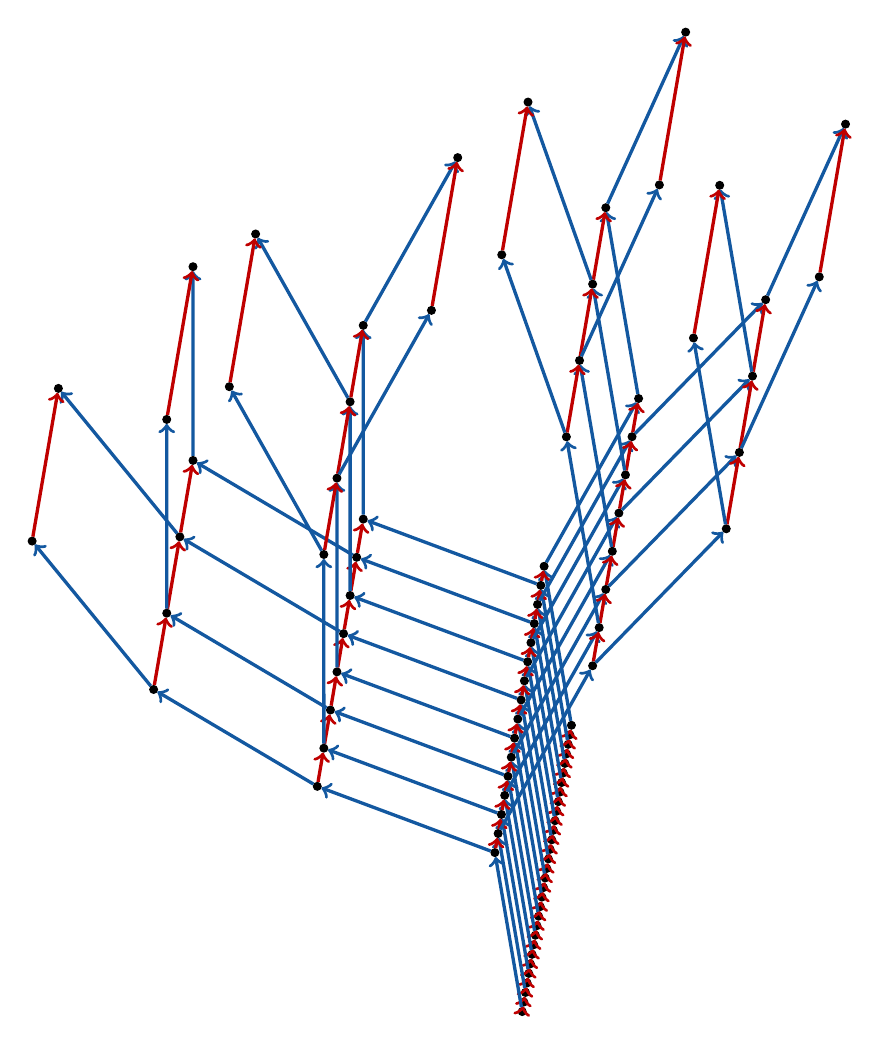
\begin{tikzpicture}
[xscale=0.4,yscale=0.41,node distance=0.5cm,
nn/.style={circle,fill,draw=black,inner sep=1pt},font=\small]
%%%%% LEVEL -1
\node[nn] (nivelm10) at (0,0) {};
\foreach \i[remember=\i as \lasti (initially 0)] in {1,...,30}
{
	\node[nn] (nivelm1\i) at ([shift=({80:0.3 cm})]nivelm1\lasti) {};
	\path[->, very thick,draw={rgb, 255:red, 191; green, 0; blue, 0 }] (nivelm1\lasti) edge (nivelm1\i);
};
%%%%% LEVEL 0
\foreach \i[remember=\i as \lasti (initially 0)] in {0,2,...,30}
{
	\node[nn] (nivel0\i) at ([shift=({100:5 cm})]nivelm1\i) {};
	\path[->, very thick,draw={rgb, 255:red, 19; green, 88; blue, 160 }] (nivelm1\i) edge (nivel0\i);
	\ifnum \i>0
	\path[->, very thick,draw={rgb, 255:red, 191; green, 0; blue, 0 }] (nivel0\lasti) edge (nivel0\i);
	\fi 
};
%%%%% LEVEL 1
\foreach \i[remember=\i as \lasti (initially 0)] in {0,4,...,30}
{
	\node[nn] (nivel1\i) at ([shift=({160:6 cm})]nivel0\i) {};
	\path[->, very thick,draw={rgb, 255:red, 19; green, 88; blue, 160 }] (nivel0\i) edge (nivel1\i);
	\ifnum \i>0
	\path[->, very thick,draw={rgb, 255:red, 191; green, 0; blue, 0 }] (nivel1\lasti) edge (nivel1\i);
	\fi 
};
\foreach \i[remember=\i as \lasti (initially 2)] in {2,6,...,30}
{
	\node[nn] (nivel1\i) at ([shift=({60:6 cm})]nivel0\i) {};
	\path[->, very thick,draw={rgb, 255:red, 19; green, 88; blue, 160 }] (nivel0\i) edge (nivel1\i);
	\ifnum \i>2
	\path[->, very thick,draw={rgb, 255:red, 191; green, 0; blue, 0 }] (nivel1\lasti) edge (nivel1\i);
	\fi 
};
%%%%% LEVEL 2
\foreach \i[remember=\i as \lasti (initially 0)] in {0,8,...,30}
{
	\node[nn] (nivel2\i) at ([shift=({150:6 cm})]nivel1\i) {};
	\path[->, very thick,draw={rgb, 255:red, 19; green, 88; blue, 160 }] (nivel1\i) edge (nivel2\i);
	\ifnum \i>0
	\path[->, very thick,draw={rgb, 255:red, 191; green, 0; blue, 0 }] (nivel2\lasti) edge (nivel2\i);
	\fi 
};
\foreach \i[remember=\i as \lasti (initially 4)] in {4,12,...,30}
{
	\node[nn] (nivel2\i) at ([shift=({90:6 cm})]nivel1\i) {};
	\path[->, very thick,draw={rgb, 255:red, 19; green, 88; blue, 160 }] (nivel1\i) edge (nivel2\i);
	\ifnum \i>4
	\path[->, very thick,draw={rgb, 255:red, 191; green, 0; blue, 0 }] (nivel2\lasti) edge (nivel2\i);
	\fi 
};
\foreach \i[remember=\i as \lasti (initially 2)] in {2,10,...,30}
{
	\node[nn] (nivel2\i) at ([shift=({45:6 cm})]nivel1\i) {};
	\path[->, very thick,draw={rgb, 255:red, 19; green, 88; blue, 160 }] (nivel1\i) edge (nivel2\i);
	\ifnum \i>2
	\path[->, very thick,draw={rgb, 255:red, 191; green, 0; blue, 0 }] (nivel2\lasti) edge (nivel2\i);
	\fi 
};
\foreach \i[remember=\i as \lasti (initially 6)] in {6,14,...,30}
{
	\node[nn] (nivel2\i) at ([shift=({100:6 cm})]nivel1\i) {};
	\path[->, very thick,draw={rgb, 255:red, 19; green, 88; blue, 160 }] (nivel1\i) edge (nivel2\i);
	\ifnum \i>6
	\path[->, very thick,draw={rgb, 255:red, 191; green, 0; blue, 0 }] (nivel2\lasti) edge (nivel2\i);
	\fi 
};
%%%% LEVEL 3
\foreach \i[remember=\i as \lasti (initially 0)] in {0,16,...,30}
{
	\node[nn] (nivel3\i) at ([shift=({130:6 cm})]nivel2\i) {};
	\path[->, very thick,draw={rgb, 255:red, 19; green, 88; blue, 160 }] (nivel2\i) edge (nivel3\i);
	\ifnum \i>0
	\path[->, very thick,draw={rgb, 255:red, 191; green, 0; blue, 0 }] (nivel3\lasti) edge (nivel3\i);
	\fi 
};
\foreach \i[remember=\i as \lasti (initially 2)] in {2,18,...,30}
{
	\node[nn] (nivel3\i) at ([shift=({100:6 cm})]nivel2\i) {};
	\path[->, very thick,draw={rgb, 255:red, 19; green, 88; blue, 160 }] (nivel2\i) edge (nivel3\i);
	\ifnum \i>2
	\path[->, very thick,draw={rgb, 255:red, 191; green, 0; blue, 0 }] (nivel3\lasti) edge (nivel3\i);
	\fi 
};
\foreach \i[remember=\i as \lasti (initially 4)] in {4,20,...,30}
{
	\node[nn] (nivel3\i) at ([shift=({120:6 cm})]nivel2\i) {};
	\path[->, very thick,draw={rgb, 255:red, 19; green, 88; blue, 160 }] (nivel2\i) edge (nivel3\i);
	\ifnum \i>4
	\path[->, very thick,draw={rgb, 255:red, 191; green, 0; blue, 0 }] (nivel3\lasti) edge (nivel3\i);
	\fi 
};
\foreach \i[remember=\i as \lasti (initially 6)] in {6,22,...,30}
{
	\node[nn] (nivel3\i) at ([shift=({110:6 cm})]nivel2\i) {};
	\path[->, very thick,draw={rgb, 255:red, 19; green, 88; blue, 160 }] (nivel2\i) edge (nivel3\i);
	\ifnum \i>6
	\path[->, very thick,draw={rgb, 255:red, 191; green, 0; blue, 0 }] (nivel3\lasti) edge (nivel3\i);
	\fi 
};
\foreach \i[remember=\i as \lasti (initially 8)] in {8,24,...,30}
{
	\node[nn] (nivel3\i) at ([shift=({90:6 cm})]nivel2\i) {};
	\path[->, very thick,draw={rgb, 255:red, 19; green, 88; blue, 160 }] (nivel2\i) edge (nivel3\i);
	\ifnum \i>8
	\path[->, very thick,draw={rgb, 255:red, 191; green, 0; blue, 0 }] (nivel3\lasti) edge (nivel3\i);
	\fi 
};
\foreach \i[remember=\i as \lasti (initially 10)] in {10,26,...,30}
{
	\node[nn] (nivel3\i) at ([shift=({65:6 cm})]nivel2\i) {};
	\path[->, very thick,draw={rgb, 255:red, 19; green, 88; blue, 160 }] (nivel2\i) edge (nivel3\i);
	\ifnum \i>10
	\path[->, very thick,draw={rgb, 255:red, 191; green, 0; blue, 0 }] (nivel3\lasti) edge (nivel3\i);
	\fi 
};
\foreach \i[remember=\i as \lasti (initially 12)] in {12,28,...,30}
{
	\node[nn] (nivel3\i) at ([shift=({60:6 cm})]nivel2\i) {};
	\path[->, very thick,draw={rgb, 255:red, 19; green, 88; blue, 160 }] (nivel2\i) edge (nivel3\i);
	\ifnum \i>12
	\path[->, very thick,draw={rgb, 255:red, 191; green, 0; blue, 0 }] (nivel3\lasti) edge (nivel3\i);
	\fi 
};
\foreach \i[remember=\i as \lasti (initially 14)] in {14,30}
{
	\node[nn] (nivel3\i) at ([shift=({65:6 cm})]nivel2\i) {};
	\path[->, very thick,draw={rgb, 255:red, 19; green, 88; blue, 160 }] (nivel2\i) edge (nivel3\i);
	\ifnum \i>14
	\path[->, very thick,draw={rgb, 255:red, 191; green, 0; blue, 0 }] (nivel3\lasti) edge (nivel3\i);
	\fi 
};
\end{tikzpicture}
\end{document}